\documentclass[]{report}
\usepackage{lmodern}
\usepackage{amssymb,amsmath}
\usepackage{ifxetex,ifluatex}
\usepackage{fixltx2e} % provides \textsubscript
\ifnum 0\ifxetex 1\fi\ifluatex 1\fi=0 % if pdftex
  \usepackage[T1]{fontenc}
  \usepackage[utf8]{inputenc}
\else % if luatex or xelatex
  \ifxetex
    \usepackage{mathspec}
  \else
    \usepackage{fontspec}
  \fi
  \defaultfontfeatures{Ligatures=TeX,Scale=MatchLowercase}
\fi
% use upquote if available, for straight quotes in verbatim environments
\IfFileExists{upquote.sty}{\usepackage{upquote}}{}
% use microtype if available
\IfFileExists{microtype.sty}{%
\usepackage{microtype}
\UseMicrotypeSet[protrusion]{basicmath} % disable protrusion for tt fonts
}{}
\usepackage{hyperref}
\hypersetup{unicode=true,
            pdftitle={PROJECT 2: PREDICTING PH},
            pdfauthor={Juliann McEachern},
            pdfborder={0 0 0},
            breaklinks=true}
\urlstyle{same}  % don't use monospace font for urls
\usepackage{graphicx,grffile}
\makeatletter
\def\maxwidth{\ifdim\Gin@nat@width>\linewidth\linewidth\else\Gin@nat@width\fi}
\def\maxheight{\ifdim\Gin@nat@height>\textheight\textheight\else\Gin@nat@height\fi}
\makeatother
% Scale images if necessary, so that they will not overflow the page
% margins by default, and it is still possible to overwrite the defaults
% using explicit options in \includegraphics[width, height, ...]{}
\setkeys{Gin}{width=\maxwidth,height=\maxheight,keepaspectratio}
\IfFileExists{parskip.sty}{%
\usepackage{parskip}
}{% else
\setlength{\parindent}{0pt}
\setlength{\parskip}{6pt plus 2pt minus 1pt}
}
\setlength{\emergencystretch}{3em}  % prevent overfull lines
\providecommand{\tightlist}{%
  \setlength{\itemsep}{0pt}\setlength{\parskip}{0pt}}
\setcounter{secnumdepth}{0}

%%% Use protect on footnotes to avoid problems with footnotes in titles
\let\rmarkdownfootnote\footnote%
\def\footnote{\protect\rmarkdownfootnote}

%%% Change title format to be more compact
\usepackage{titling}

% Create subtitle command for use in maketitle
\providecommand{\subtitle}[1]{
  \posttitle{
    \begin{center}\large#1\end{center}
    }
}

\setlength{\droptitle}{-2em}

  \title{PROJECT 2: PREDICTING PH}
    \pretitle{\vspace{\droptitle}\centering\huge}
  \posttitle{\par}
    \author{Juliann McEachern}
    \preauthor{\centering\large\emph}
  \postauthor{\par}
      \predate{\centering\large\emph}
  \postdate{\par}
    \date{10 December 2019}

% set plain style for page numbers
\usepackage[margin=1in]{geometry}
\usepackage{fancyhdr}
\pagestyle{fancy}
\fancyhead[LE,RO]{\textbf{Group 2}}
\fancyhead[RE,LO]{\textbf{Project 2: Predicting PH}}
\raggedbottom
\setlength{\parskip}{1em}

% change font
\usepackage{fontspec}
\setmainfont{Arial}

% format titles 
\usepackage{xcolor}
\usepackage{sectsty}
\usepackage{etoolbox}
\usepackage{titling}
\definecolor{prettyblue}{RGB}{84, 144, 240}
\definecolor{bluegray}{RGB}{98, 107, 115}
\pretitle{\begin{center}\Huge\color{prettyblue}\textbf}
\posttitle{\par\LARGE\color{gray}DATA 624 - Predictive Analytics\linebreak Group 2\end{center}}
\preauthor{\begin{center}\large\textbf{Group Members:}\linebreak\textit}
\postauthor{\end{center}}

% Format chapter output
\usepackage{titlesec}
\titleclass{\part}{top}
\titleclass{\chapter}{straight}
\titleformat{\chapter}
  {\normalfont\color{prettyblue}\LARGE\bfseries}{\thechapter}{1em}{}
\titlespacing*{\chapter}{0pt}{3.5ex plus 1ex minus .2ex}{2.3ex plus .2ex}


% create color block quotes
\usepackage{tcolorbox}
\newtcolorbox{myquote}{colback=purple!05!white, colframe=purple!75!black}
\renewenvironment{quote}{\begin{myquote}}{\end{myquote}}

% kable 
\usepackage{tabu}


% multicolumn
\usepackage{multicol}

% bullets
\newenvironment{tight_enumerate}{
\begin{enumerate}
  \setlength{\itemsep}{0pt}
  \setlength{\parskip}{0pt}
  }{\end{enumerate}}
  
\newenvironment{tight_itemize}{
\begin{itemize}
  \setlength{\topsep}{0pt}
  \setlength{\itemsep}{0pt}
  \setlength{\parskip}{0pt}
  \setlength{\parsep}{0pt}
  }{\end{itemize}}

\usepackage{paralist}

%hyperlink
\usepackage{hyperref}
\hypersetup{
    colorlinks=true,
    linkcolor=bluegray,
    filecolor=magenta,      
    urlcolor=cyan}

\usepackage{graphicx}
\usepackage{wrapfig}
\usepackage{booktabs}
\definecolor{yale}{RGB}{13,77,146}
\usepackage[font={color=yale,bf,scriptsize},figurename=Fig.,belowskip=0pt,aboveskip=0pt]{caption}
\usepackage{floatrow}
\floatsetup[figure]{capposition=below}
\setlength{\abovecaptionskip}{1pt}
\setlength{\belowcaptionskip}{1pt}
\setlength{\textfloatsep}{3pt plus 0.5pt minus 0.5pt}
\setlength{\intextsep}{3pt plus 1.0pt minus 1.0pt}
\usepackage{booktabs}
\usepackage{longtable}
\usepackage{array}
\usepackage{multirow}
\usepackage{wrapfig}
\usepackage{float}
\usepackage{colortbl}
\usepackage{pdflscape}
\usepackage{tabu}
\usepackage{threeparttable}
\usepackage{threeparttablex}
\usepackage[normalem]{ulem}
\usepackage{makecell}
\usepackage{xcolor}

\begin{document}
\maketitle

{
\setcounter{tocdepth}{1}
\tableofcontents
}
\thispagestyle{empty}
\newpage
\clearpage
\pagenumbering{arabic}

\hypertarget{intro}{%
\chapter*{Introduction}\label{intro}}
\addcontentsline{toc}{chapter}{Introduction}

This project is designed to evaluate production data from a beverage
manufacturing company. Our assignment is to predict \texttt{PH}, a Key
Performance Indicator (KPI), with a high degree of accuracy through
predictive modeling. After thorough examination, we approached this task
by splitting the provided data into training and test sets. We evaluated
several models on this split and found that
\textbf{what-ever-worked-best} method yielded the best results.

Each group member worked individually to create their own solution. We
built our final submission by collaboratively evaluating and combining
each others' approaches. Our introduction should further outline
individual responsibilities. For example, \textbf{so-and-so} was
responsible for \textbf{xyz task}.

For replication and grading purposes, we made our code avaliable in the
appendix section. This code, along with the provided data, score-set
results, and individual contributions, can also be accessed through our
group github repository:

\begin{compactitem}
  \item \href{https://github.com/JeremyOBrien16/CUNY_DATA_624/tree/master/Project_Two}{Pretend I'm a working link to R Source Code}
  \item \href{https://github.com/JeremyOBrien16/CUNY_DATA_624/tree/master/Project_Two}{Pretend I'm a working link to Provided Data}
  \item \href{https://github.com/JeremyOBrien16/CUNY_DATA_624/tree/master/Project_Two}{Pretend I'm a working link to Excel Results}
  \item \href{https://github.com/JeremyOBrien16/CUNY_DATA_624/tree/master/Project_Two}{Pretend I'm a working link to Individual Work}
\end{compactitem}

\hypertarget{data-exploration}{%
\chapter{Data Exploration}\label{data-exploration}}

The beverage manufacturing production dataset contained 33
columns/variables and 2,571 rows/cases. In our initial review, we found
that the response variable, \texttt{PH}, had four missing observations.
We choose to drop the complete cases of all observations with null data
in the target as they accounted for such a small proportion (\textless{}
0.002\%) of the observations.

We also identified that 94\% of the predictor variables had missing data
points. Despite this high occurance, the NA values in the majority of
these predictors accounted for less than 1\% of the total observations.
Only eleven variables were missing more than 1\% of data. The table
below shows the top variables with the most observations missing:

\begin{table}[H]
\centering\begingroup\fontsize{8}{10}\selectfont

\begin{tabular}{lrrrrrrrrrr}
\toprule
\textbf{ } & \textbf{MFR} & \textbf{BrandCode} & \textbf{FillerSpeed} & \textbf{PCVolume} & \textbf{PSCCO2} & \textbf{FillOunces} & \textbf{PSC} & \textbf{CarbPressure1} & \textbf{HydPressure4} & \textbf{CarbPressure}\\
\midrule
\rowcolor{gray!6}  n & 208.0 & 120.0 & 54.0 & 39.0 & 39.0 & 38.0 & 33.0 & 32.0 & 28.0 & 27.0\\
\% & 8.1 & 4.7 & 2.1 & 1.5 & 1.5 & 1.5 & 1.3 & 1.2 & 1.1 & 1.1\\
\bottomrule
\end{tabular}
\endgroup{}
\end{table}

\hypertarget{response-variable}{%
\section{Response Variable}\label{response-variable}}

Understanding the influence pH has on our predictors is key to building
an accurate predictive model. pH is a measure of acidity/alkalinity that
must conform in a critical range. The value of pH ranges from 0 to 14,
where 0 is acidic, 7 is neutral, and 14 is basic.

\newpage

The plots below show the distribution of \texttt{pH} in our data. The
histogram shows us this variable follows a somewhat normal pattern and
is centered around 8.6. The boxplots also allows us to better visualize
the outliers within our target variable. We viewed \texttt{pH} (middle)
and \texttt{pH} by \texttt{BrandCode} (right) to examine the differences
in distribution and relationship between these variables. Brand D has
the highest median \texttt{pH} and brand C has the lowest. Brand C also
appears to have the largest range in \texttt{pH} values.

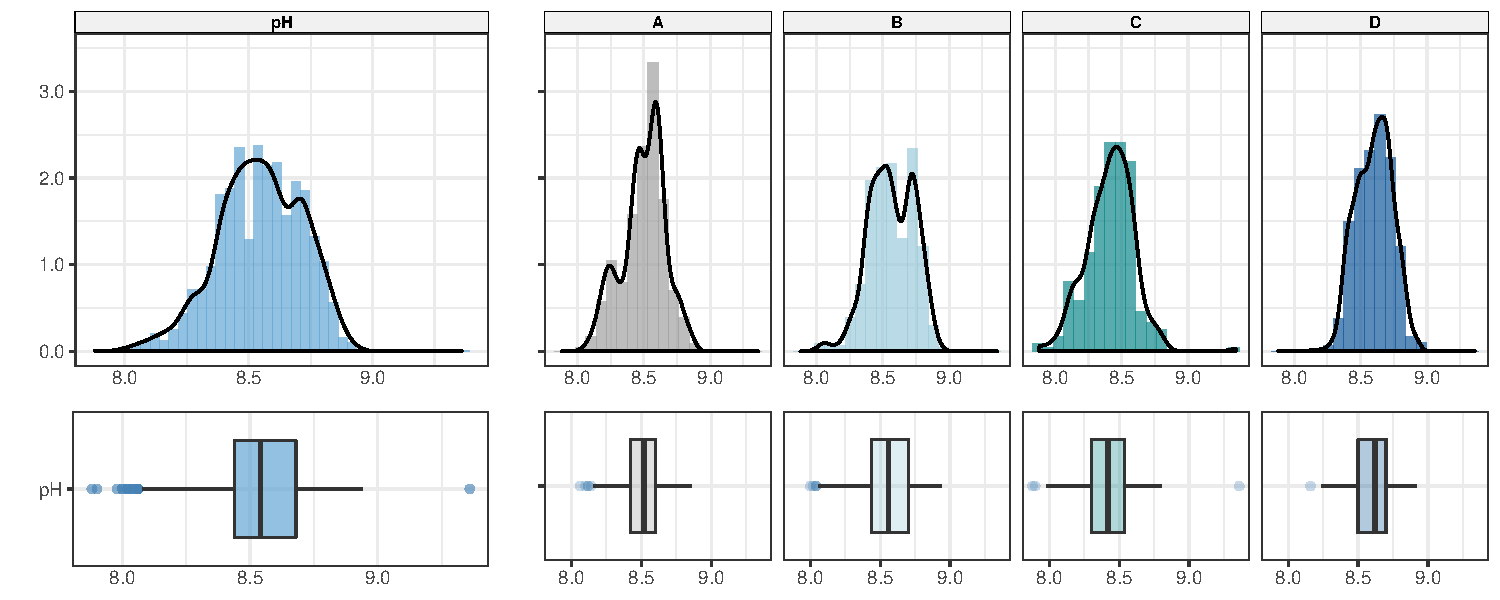
\includegraphics{Proj2-JM_files/figure-latex/unnamed-chunk-2-1.pdf}

\hypertarget{predictor-variables}{%
\section{Predictor Variables}\label{predictor-variables}}

Many of our predictors also contain outliers and have a skewed
distribution. The boxplots below help us visualize this spread of our
numeric predictor variables.

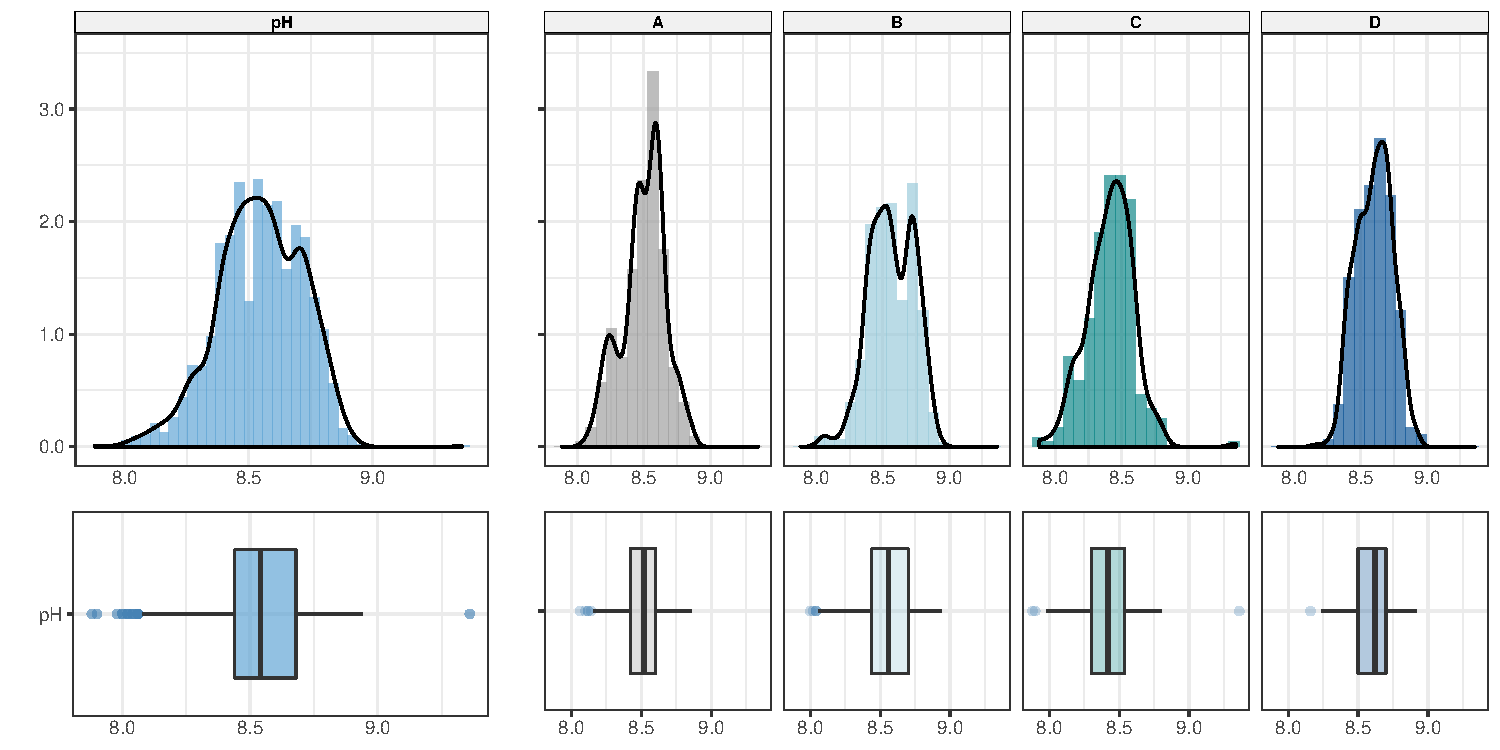
\includegraphics{Proj2-JM_files/figure-latex/unnamed-chunk-3-1.pdf}

We examined the predictor variables with outliers in a scatterplot
against our target, \texttt{pH} to better understand predictor and
response relationship. The outliers, highlighted in blue, further show
which predictors have a heavy-tail distribution. We can also identify
many variables with strong outlier patterns, suggesting a high degree of
variability within certain measurements.

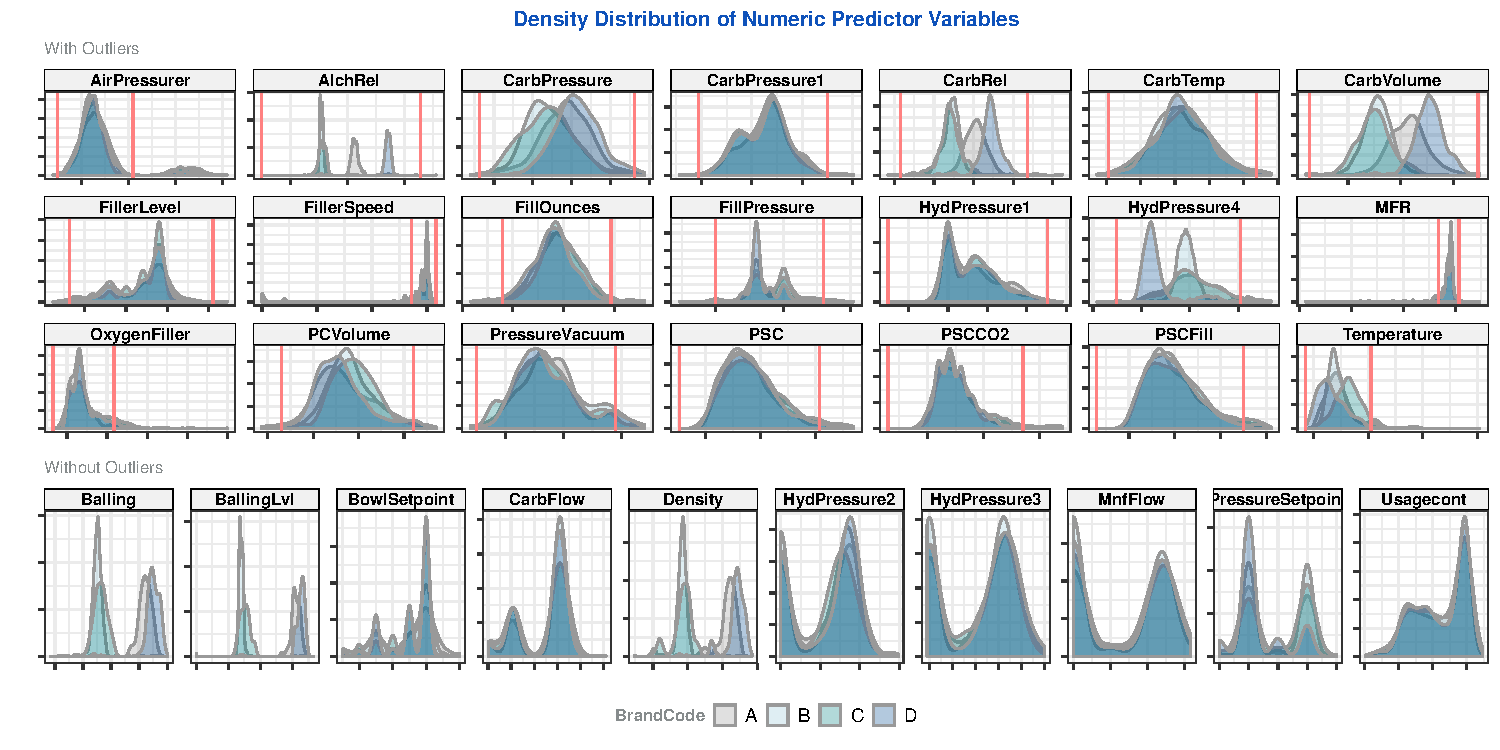
\includegraphics{Proj2-JM_files/figure-latex/unnamed-chunk-4-1.pdf}

For example, \texttt{AirPressurer} shows one of the more distinct
patterns. This variable appears bifurcated with a clear split between
normal and extreme values. \texttt{MFR} also shows an interesting
pattern. The outliers have a weak, negative linear relationship with
\texttt{pH}, but the non-outliers have no linear relationship and follow
a straight, vertical line.

\hypertarget{correlation}{%
\section{Correlation}\label{correlation}}

9 of our numeric predictor appear heavily related, with correlation
values exceeding \(\pm{0.75}\). The full correlation matrix can be
viewed in the appendix section. \emph{Revisit section to add more text}

\begin{table}[H]

\caption{\label{tab:unnamed-chunk-6}Highly Correlated Predictors}
\fontsize{8}{10}\selectfont
\begin{tabular}{lll>{\bfseries}llll}
\toprule
\textbf{V1} & \textbf{V2} & \textbf{COR} & \textbf{|} & \textbf{V1  } & \textbf{V2 } & \textbf{COR }\\
\midrule
\rowcolor{gray!6}  AlchRel & BallingLvl & 0.93 & | & CarbVolume & AlchRel & 0.78\\
AlchRel & CarbRel & 0.84 & | & CarbVolume & Density & 0.76\\
\rowcolor{gray!6}  Balling & BallingLvl & 0.98 & | & Density & Balling & 0.95\\
Balling & AlchRel & 0.92 & | & Density & BallingLvl & 0.95\\
\rowcolor{gray!6}  Balling & CarbRel & 0.82 & | & Density & AlchRel & 0.90\\
\addlinespace
CarbPressure & CarbTemp & 0.81 & | & Density & CarbRel & 0.82\\
\rowcolor{gray!6}  CarbRel & BallingLvl & 0.84 & | & FillerLevel & BowlSetpoint & 0.95\\
CarbVolume & CarbRel & 0.79 & | & FillerSpeed & MFR & 0.93\\
\rowcolor{gray!6}  CarbVolume & Balling & 0.78 & | & HydPressure2 & HydPressure3 & 0.93\\
CarbVolume & BallingLvl & 0.78 & | & MnfFlow & HydPressure3 & 0.76\\
\bottomrule
\end{tabular}
\end{table}

\hypertarget{data-preparation}{%
\chapter{Data Preparation}\label{data-preparation}}

Decision tree and boosted models are robust against the affect of
multicollineraty, outliers, and missing values. \emph{Tranformation
approaches will vary as we play with model. Visit this section later.}

We divided data using an 80/20 split to create a train and test set. All
models will incorporate k-folds cross-validation across 10 folds to
protect against overfitting the data.

\hypertarget{data-imputation}{%
\section{Data Imputation}\label{data-imputation}}

We choose to handle missing data in our predictor variables using
multiple imputations. We applied a Multiple Imputation by Chained
Equations (MICE) algorthim, which uses sequential regression to fill in
the data across all the incomplete cases (including categorical data).

\emph{We can also use this same approach to handle outliers (linear
model) by setting their value to \texttt{NA} and predicticting a value
within the expected range.}

\hypertarget{pre-processing}{%
\section{Pre-Processing}\label{pre-processing}}

\emph{Test the effect of pre-processing methods to maximize the success
of our tree and non-tree models. Not currently adding data
transformations but may revist: ie. scale data for PLS. }

For linear models, we removed the predictor \texttt{HydPressure1} as it
contained near-zero variance. \texttt{HydPressure3}, \texttt{Balling},
\texttt{BallingLvl}, \texttt{FillerSpeed}, \texttt{FillerLevel}, and
\texttt{Density} were also removed due to large absolute correlations
with other variables.

\hypertarget{predictive-modeling}{%
\chapter{Predictive Modeling}\label{predictive-modeling}}

Only attempted 1 model thus far: MARS. Text explination to come.

\hypertarget{mars-model}{%
\section{MARS Model}\label{mars-model}}

Explain text here. Text text text text text text text text text text
text text text text text text text text text text text text text text
text text text text text text text text text text text text text text
text text text text text text text text text text text text text text
text text text text text text text text text.

\textbf{MARS CV RMSE:}
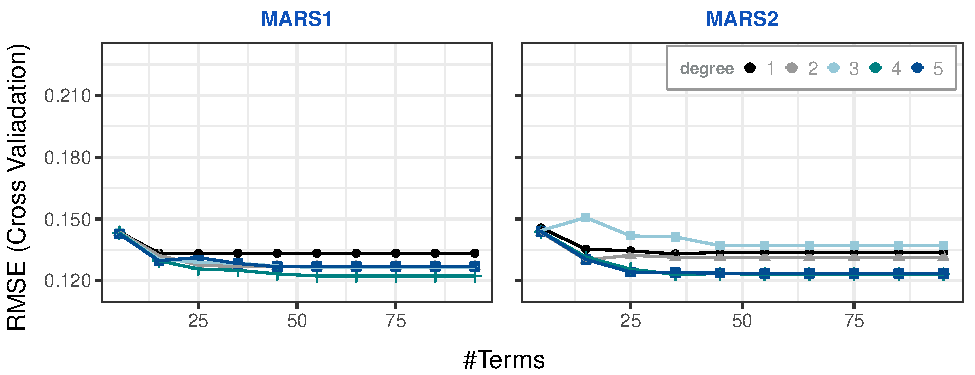
\includegraphics{Proj2-JM_files/figure-latex/unnamed-chunk-7-1.pdf}

\textbf{Train Accuracy: }

\begin{table}[H]
\centering\begingroup\fontsize{8}{10}\selectfont

\begin{tabular}{r|r|r}
\hline
RMSE & Rsquared & MAE\\
\hline
\rowcolor{gray!6}  0.1229609 & 0.5076279 & 0.0915898\\
\hline
\end{tabular}
\endgroup{}
\end{table}

\textbf{Test Accuracy:}

\begin{table}[H]
\centering\begingroup\fontsize{8}{10}\selectfont

\begin{tabular}{r|r|r}
\hline
RMSE & Rsquared & MAE\\
\hline
\rowcolor{gray!6}  0.1220149 & 0.4911614 & 0.0904218\\
\hline
\end{tabular}
\endgroup{}
\end{table}

Variable Importance:

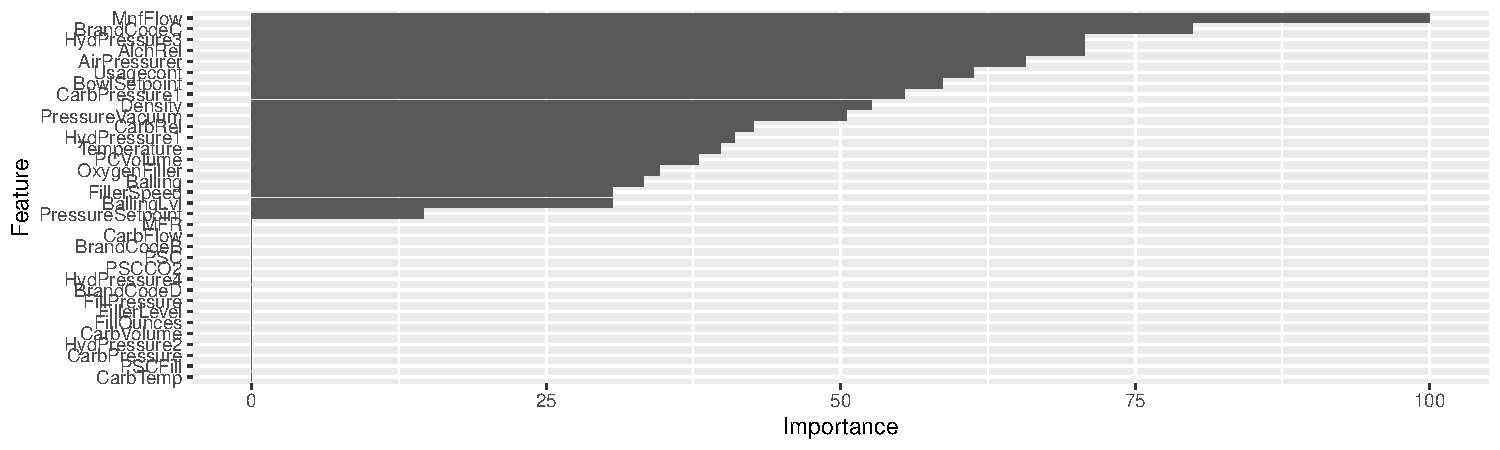
\includegraphics{Proj2-JM_files/figure-latex/unnamed-chunk-10-1.pdf}

\hypertarget{train}{%
\section{Train}\label{train}}

Train text.

\hypertarget{test}{%
\section{Test}\label{test}}

Test text.

\hypertarget{discussion}{%
\chapter{Discussion}\label{discussion}}

Eval text. The end.

\hypertarget{conclusion}{%
\chapter{Conclusion}\label{conclusion}}

sfasdfs

\hypertarget{Appendix}{%
\chapter*{Appendix}\label{Appendix}}
\addcontentsline{toc}{chapter}{Appendix}

\hypertarget{summary-statistics}{%
\section{Summary Statistics}\label{summary-statistics}}

\begin{table}[H]
\centering\begingroup\fontsize{8}{10}\selectfont

\begin{tabular}{lrrrrrrrrrrrrr}
\toprule
  & vars & n & mean & sd & median & trimmed & mad & min & max & range & skew & kurtosis & se\\
\midrule
\rowcolor{gray!6}  BrandCode* & 1 & 2447 & 2.5 & 1.0 & 2.0 & 2.5 & 0.0 & 1.0 & 4.0 & 3.0 & 0.4 & -1.1 & 0.0\\
CarbVolume & 2 & 2557 & 5.4 & 0.1 & 5.3 & 5.4 & 0.1 & 5.0 & 5.7 & 0.7 & 0.4 & -0.5 & 0.0\\
\rowcolor{gray!6}  FillOunces & 3 & 2529 & 24.0 & 0.1 & 24.0 & 24.0 & 0.1 & 23.6 & 24.3 & 0.7 & 0.0 & 0.9 & 0.0\\
PCVolume & 4 & 2528 & 0.3 & 0.1 & 0.3 & 0.3 & 0.1 & 0.1 & 0.5 & 0.4 & 0.3 & 0.7 & 0.0\\
\rowcolor{gray!6}  CarbPressure & 5 & 2540 & 68.2 & 3.5 & 68.2 & 68.1 & 3.6 & 57.0 & 79.4 & 22.4 & 0.2 & 0.0 & 0.1\\
\addlinespace
CarbTemp & 6 & 2541 & 141.1 & 4.0 & 140.8 & 141.0 & 3.9 & 128.6 & 154.0 & 25.4 & 0.2 & 0.2 & 0.1\\
\rowcolor{gray!6}  PSC & 7 & 2534 & 0.1 & 0.0 & 0.1 & 0.1 & 0.0 & 0.0 & 0.3 & 0.3 & 0.9 & 0.7 & 0.0\\
PSCFill & 8 & 2544 & 0.2 & 0.1 & 0.2 & 0.2 & 0.1 & 0.0 & 0.6 & 0.6 & 0.9 & 0.8 & 0.0\\
\rowcolor{gray!6}  PSCCO2 & 9 & 2528 & 0.1 & 0.0 & 0.0 & 0.0 & 0.0 & 0.0 & 0.2 & 0.2 & 1.7 & 3.7 & 0.0\\
MnfFlow & 10 & 2567 & 24.6 & 119.5 & 70.2 & 21.1 & 161.6 & -100.2 & 229.4 & 329.6 & 0.0 & -1.9 & 2.4\\
\addlinespace
\rowcolor{gray!6}  CarbPressure1 & 11 & 2535 & 122.6 & 4.7 & 123.2 & 122.5 & 4.4 & 105.6 & 140.2 & 34.6 & 0.0 & 0.1 & 0.1\\
FillPressure & 12 & 2549 & 47.9 & 3.2 & 46.4 & 47.7 & 2.4 & 34.6 & 60.4 & 25.8 & 0.5 & 1.4 & 0.1\\
\rowcolor{gray!6}  HydPressure1 & 13 & 2556 & 12.5 & 12.4 & 11.4 & 10.9 & 16.9 & -0.8 & 58.0 & 58.8 & 0.8 & -0.1 & 0.2\\
HydPressure2 & 14 & 2552 & 21.0 & 16.4 & 28.6 & 21.1 & 13.3 & 0.0 & 59.4 & 59.4 & -0.3 & -1.6 & 0.3\\
\rowcolor{gray!6}  HydPressure3 & 15 & 2552 & 20.5 & 16.0 & 27.6 & 20.5 & 13.8 & -1.2 & 50.0 & 51.2 & -0.3 & -1.6 & 0.3\\
\addlinespace
HydPressure4 & 16 & 2539 & 96.3 & 13.1 & 96.0 & 95.5 & 11.9 & 62.0 & 142.0 & 80.0 & 0.6 & 0.6 & 0.3\\
\rowcolor{gray!6}  FillerLevel & 17 & 2551 & 109.3 & 15.7 & 118.4 & 111.0 & 9.2 & 55.8 & 161.2 & 105.4 & -0.8 & 0.0 & 0.3\\
FillerSpeed & 18 & 2513 & 3688.1 & 769.6 & 3982.0 & 3920.2 & 47.4 & 998.0 & 4030.0 & 3032.0 & -2.9 & 6.8 & 15.4\\
\rowcolor{gray!6}  Temperature & 19 & 2555 & 66.0 & 1.4 & 65.6 & 65.8 & 0.9 & 63.6 & 76.2 & 12.6 & 2.4 & 10.3 & 0.0\\
Usagecont & 20 & 2562 & 21.0 & 3.0 & 21.8 & 21.3 & 3.2 & 12.1 & 25.9 & 13.8 & -0.5 & -1.0 & 0.1\\
\addlinespace
\rowcolor{gray!6}  CarbFlow & 21 & 2565 & 2472.1 & 1070.4 & 3030.0 & 2604.2 & 323.2 & 26.0 & 5104.0 & 5078.0 & -1.0 & -0.6 & 21.1\\
Density & 22 & 2567 & 1.2 & 0.4 & 1.0 & 1.2 & 0.1 & 0.2 & 1.9 & 1.7 & 0.5 & -1.2 & 0.0\\
\rowcolor{gray!6}  MFR & 23 & 2359 & 704.0 & 73.9 & 724.0 & 718.2 & 15.4 & 31.4 & 868.6 & 837.2 & -5.1 & 30.5 & 1.5\\
Balling & 24 & 2567 & 2.2 & 0.9 & 1.6 & 2.1 & 0.4 & 0.2 & 4.0 & 3.9 & 0.6 & -1.4 & 0.0\\
\rowcolor{gray!6}  PressureVacuum & 25 & 2567 & -5.2 & 0.6 & -5.4 & -5.3 & 0.6 & -6.6 & -3.6 & 3.0 & 0.5 & 0.0 & 0.0\\
\addlinespace
PH & 26 & 2567 & 8.5 & 0.2 & 8.5 & 8.6 & 0.2 & 7.9 & 9.4 & 1.5 & -0.3 & 0.1 & 0.0\\
\rowcolor{gray!6}  OxygenFiller & 27 & 2556 & 0.0 & 0.0 & 0.0 & 0.0 & 0.0 & 0.0 & 0.4 & 0.4 & 2.4 & 8.8 & 0.0\\
BowlSetpoint & 28 & 2565 & 109.3 & 15.3 & 120.0 & 111.4 & 0.0 & 70.0 & 140.0 & 70.0 & -1.0 & -0.1 & 0.3\\
\rowcolor{gray!6}  PressureSetpoint & 29 & 2555 & 47.6 & 2.0 & 46.0 & 47.6 & 0.0 & 44.0 & 52.0 & 8.0 & 0.2 & -1.6 & 0.0\\
AirPressurer & 30 & 2567 & 142.8 & 1.2 & 142.6 & 142.6 & 0.6 & 140.8 & 148.2 & 7.4 & 2.3 & 4.7 & 0.0\\
\addlinespace
\rowcolor{gray!6}  AlchRel & 31 & 2560 & 6.9 & 0.5 & 6.6 & 6.8 & 0.1 & 5.3 & 8.6 & 3.3 & 0.9 & -0.9 & 0.0\\
CarbRel & 32 & 2559 & 5.4 & 0.1 & 5.4 & 5.4 & 0.1 & 5.0 & 6.1 & 1.1 & 0.5 & -0.3 & 0.0\\
\rowcolor{gray!6}  BallingLvl & 33 & 2566 & 2.1 & 0.9 & 1.5 & 2.0 & 0.2 & 0.0 & 3.7 & 3.7 & 0.6 & -1.5 & 0.0\\
\bottomrule
\end{tabular}
\endgroup{}
\end{table}

\hypertarget{correlation-matrix}{%
\section{Correlation Matrix}\label{correlation-matrix}}

\begin{center}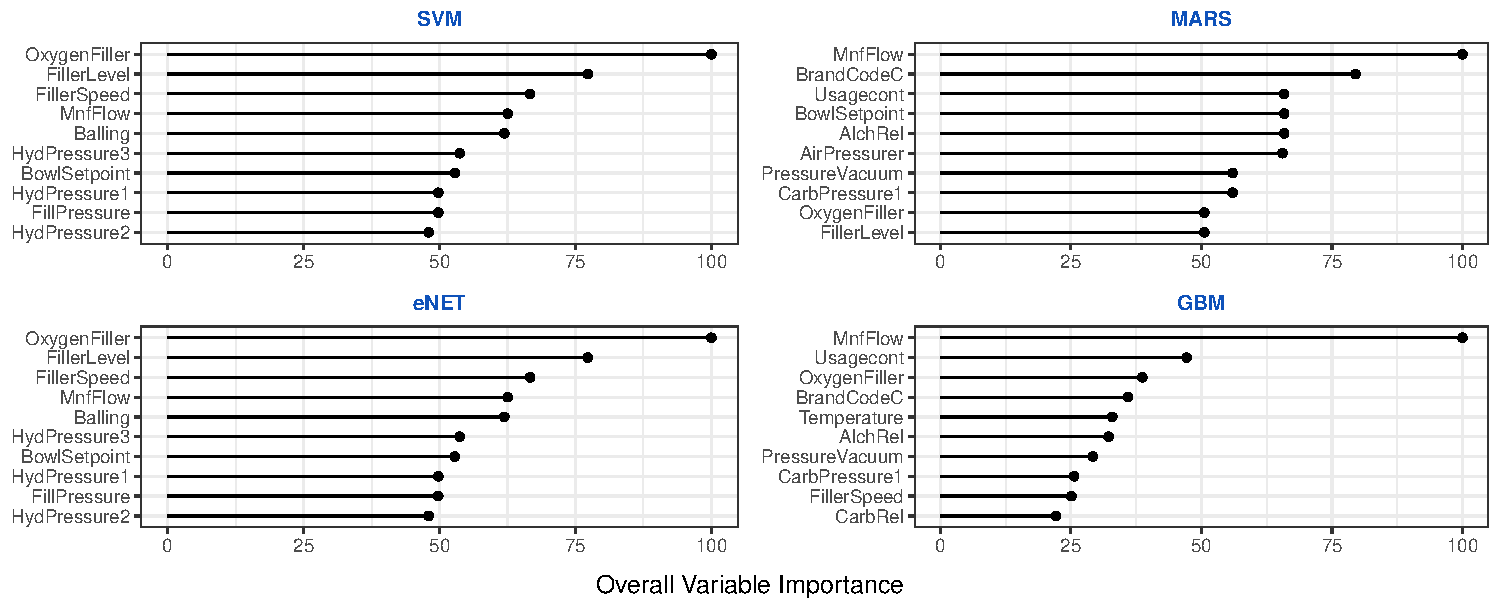
\includegraphics{Proj2-JM_files/figure-latex/unnamed-chunk-12-1} \end{center}


\end{document}
